\documentclass[12pt]{article}
\usepackage{amsmath, amssymb, amsthm}
\usepackage{import}
\usepackage{pdfpages}
\usepackage{transparent}
\usepackage{xcolor}
\usepackage{graphicx, epstopdf}

\usepackage{fancyhdr}
\usepackage[framed, numbered]{matlab-prettifier}

\fancyhf{}
\pagestyle{fancy}
\lhead{Carrera}
\rhead{\thepage}

\setlength\parindent{0pt}
\numberwithin{equation}{section}

\usepackage{titlesec}
\titleformat{\section}
{\normalfont\Large\bfseries}{Exercise~\thesection}{1em}{}

\newcommand{\incfig}[2][1]{%
  \def\svgwidth{#1\columnwidth}
  \import{./figures/}{#2.pdf_tex}
}

\newcommand{\RE}{\mathrm{Re}}
\newcommand{\IM}{\mathrm{Im}}

\newcommand\ddfrac[2]{\frac{\displaystyle #1}{\displaystyle #2}}

\pdfsuppresswarningpagegroup=1

\author{Adam Carrera}
\date{February 24 , 2021}
\title{MECH 3340 - Assignment \#3}

\begin{document}
  \maketitle

  \section{}

  Resolve feedback loop between blocks $ 1/s $ and $ 8. $

  \[
      \frac{1/s}{1+8/s} = \ddfrac{1/s}{\frac{s+8}{s}} = \frac{1}{s+8}
    .\]

  Blocks $ 4, 1/s $ are in series with the sum of $ G(s), 1/(s+8). $

  \[
      (4/s + G(s))\frac{1}{s+8}
    .\]

  Which is in a feedback loop with $ 6. $

  \[
      \ddfrac{(4/s + G(s))\frac{1}{s+8}}{1 + \frac{6}{s+8} \left( 4/s + G(s) \right) }
    .\]

  \[
      = \ddfrac{\frac{4}{s(s+8)} + \frac{G(s)}{s + 8}}{\frac{s(s+8) + 24 + sG(s)}{s(s + 8)}}
    .\]

  \begin{equation}
    \frac{X(s)}{F(s)} = \frac{4 + sG(s)}{s ^2 + (G(s) + 8)s + 24}
  \end{equation}

  \newpage



  \section{}

  Note that $ G_n, H_n $ are functions of $ s. $

  \subsection{$ V(s) = 0 $}

  Combine $ G_2, H_2 $ using feedback. This is in series with $ G_1. $

  \[
      \frac{G_1 G_2}{1 + G_2H_2}
    .\]

  Finally, combine the above with $ H_1 $ using feedback.

  \[
      \ddfrac{\frac{G_1 G_2}{1 + G_2H_2}}{1 + \frac{G_1G_2H_1}{1 + G_2H_2}}
    .\]

  \begin{equation}
    \frac{Y(s)}{U(s)} = \frac{G_1(s)G_2(s)}{1 + G_2(s)H_2(s) + G_1(s)G_2(s)H_1(s)}
  \end{equation}

  \subsection{$ U(s) = 0. $}

  \begin{figure}
    \centering
    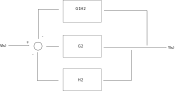
\includegraphics[width=0.85\textwidth]{figures/problem2.png}
    \caption{Equivalent block diagram derived from $ U(s) = 0. $ (Exercise 2)}
    \label{fig:problem2}
  \end{figure}

  With $ U(s) = 0, $ we can draw an equivalent block diagram (see Figure \ref{fig:problem2}). Combine $ G_2, H_2 $ using feedback.

  \[
      \frac{G_2}{1 + G_2H_2}
    .\]

  Finally, combine the above result with $ G_1H_2 $ using feedback.

  \[
      \ddfrac{\frac{G_2}{1 + G_2H_2}}{1 + \frac{G_1G_2H_1}{1 + G_2H_2}}
    .\]

  \begin{equation}
    \frac{Y(s)}{V(s)} = \frac{G_2(s)}{1 + G_2(s)H_2(s) + G_1(s)G_2(s)H_1(s)}
  \end{equation}



  \section{}

  Given,

  \[
      5 \ddot x + 3 \dot x + 7 x = 10f(t) - 4g(t)
    .\]

  Take the laplace transform of both sides,

  \[
      \left( 5 s ^2 + 3s + 7 \right) X(s) = 10F(s) - 4G(s)
    .\]

  \begin{equation}\label{eqn:eq1}
    X(s) = \frac{10}{\left( 5 s ^2 + 3s + 7 \right)}F(s) - \frac{4}{\left( 5 s ^2 + 3s + 7 \right)} G(s)
  \end{equation}

  Let,

  \[
      H_1 = \frac{10}{\left( 5 s ^2 + 3s + 7 \right)}, \quad H_2 = \frac{4}{\left( 5 s ^2 + 3s + 7 \right)}
    .\]

  Equation (\ref{eqn:eq1}) can be represented in block diagram form. See Figure \ref{fig:problem3}.

  \begin{figure}
    \centering
    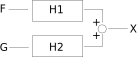
\includegraphics[width=0.85\textwidth]{figures/problem3.png}
    \caption{Block diagram solution for Exercise 3}
    \label{fig:problem3}
  \end{figure}

  \newpage


  \section{}

  Given the system,

  \[
      \begin{aligned}
        2 \ddot y + \dot y + y &= z \\
        \dot z + 3z + y &= f(t)
      \end{aligned}
    \]

  Let,

  \[
    x =
    \begin{bmatrix}
      y \\ \dot y \\ z
    \end{bmatrix}
      =
    \begin{bmatrix}
      x_1 \\ x_2 \\ x_3
    \end{bmatrix}
    .\]

  \[
      \Rightarrow \dot x =
      \begin{bmatrix}
        x_2 \\ x_3 - x_2 - x_1 \\ -x_1 -3x_3 + f(t)
      \end{bmatrix}
    .\]

  Write $ \dot x $ in the form of $ \dot x = Ax + Bu. $

  \begin{equation}
    \dot x =
    \begin{bmatrix}
      0 & 1 & 0 \\
      -1 & -1 & 1 \\
      -1 & 0 & -3
    \end{bmatrix}
    \begin{bmatrix}
      x_1 \\ x_2 \\ x_3
    \end{bmatrix} +
    \begin{bmatrix}
      0 \\ 0 \\ 1
    \end{bmatrix} f(t)
  \end{equation}

  \newpage


  \section{}

  Listing 1 and Figure \ref{fig:problem5} show the matlab solution and resulting plot, respectively.

  \lstinputlisting[style=Matlab-editor, caption = {Script for Problem 5, a system and input are defined and simulated}]{MATLAB/problem5.m}

  \begin{figure}[ht!]
    \centering
    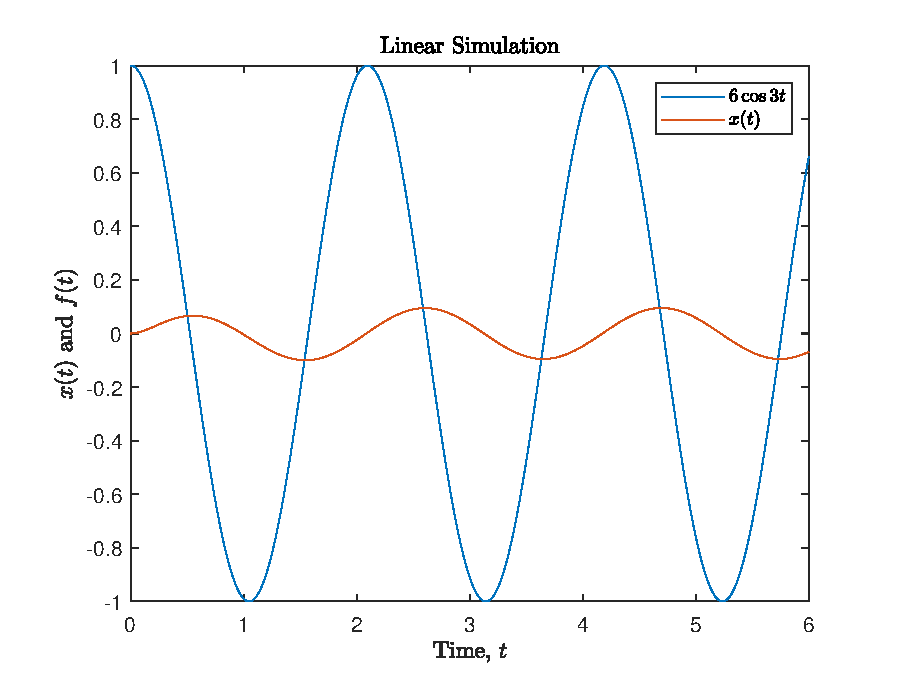
\includegraphics[width=\textwidth]{figures/problem5.eps}
    \caption{System Response versus Input Force}
    \label{fig:problem5}
  \end{figure}

  \newpage
  \section{}

  Assume that $ D(s) = 0. $ The result from listing 2 is,

  \begin{equation}
    \frac{C(s)}{R(s)} = \frac{6}{12s^3 + 11s^2 + 12s + 6}
  \end{equation}

  \newpage

  \lstinputlisting[style=Matlab-editor, caption = {Script for Problem 6, Transfer function blocks are defined and block diagram algebra is preformed}]{MATLAB/problem6.m}

  \begin{figure}
    \centering
    \includegraphics[width=0.85\textwidth]{figures/problem6output}
    \caption{Output of Listing 2}
    \label{fig:problem6output}
  \end{figure}

  \newpage

  \section{}

  Calculate $ C \left( sI - A \right)^{-1}B + D $ by hand,

  \[
      (sI - A)^{-1} =
      \begin{bmatrix}
        s & -1 \\
        1/2 & s + 1
      \end{bmatrix}^{-1}
    \]

  \[
      = \frac{1}{s(s + 1) + 1/2}
      \begin{bmatrix}
        s + 1 & 1 \\
        -1/2 & s
      \end{bmatrix}
    .\]

  Multiply the above result by $ \begin{bmatrix} 0 & 1 \end{bmatrix} $ and $ \begin{bmatrix} 0 \\ 2\end{bmatrix}. $


  \[
      \frac{1}{s(s + 1) + 1/2}
      \begin{bmatrix}
        -1/2 & s
      \end{bmatrix}
      \begin{bmatrix}
        0 \\ 2
      \end{bmatrix}
    .\]

  Which gives us,

  \begin{equation}
    C \left( sI - A \right)^{-1}B + D = \frac{2s}{s^2 + s + 1/2}
  \end{equation}

  We can check our answer in matlab with listing 3.

  \newpage

  \lstinputlisting[style=Matlab-editor, caption = {Script for problem 7, conversion from state space to transfer function}]{MATLAB/problem7.m}

  \begin{figure}
    \centering
    \includegraphics[width = 0.85\textwidth]{figures/problem7output}
    \caption{Output of Listing 3}
    \label{fig:problem7}
  \end{figure}

\end{document}
